% $Header: /data/cvsroot/Courses/OnlineLearning/talks/talk1/talk1.tex,v 1.5 2006/01/11 03:23:33 yfreund Exp $

%\documentclass{beamer}
\documentclass[handout]{beamer}
% This file is a solution template for:

% - Giving a talk on some subject.
% - The talk is between 15min and 45min long.
% - Style is ornate.

% Copyright 2004 by Till Tantau <tantau@users.sourceforge.net>.
%
% In principle, this file can be redistributed and/or modified under
% the terms of the GNU Public License, version 2.
%
% However, this file is supposed to be a template to be modified
% for your own needs. For this reason, if you use this file as a
% template and not specifically distribute it as part of a another
% package/program, I grant the extra permission to freely copy and
% modify this file as you see fit and even to delete this copyright
% notice. 


\mode<presentation>
{
  \usetheme{Montpellier}

  %\setbeamercovered{transparent}
  % or whatever (possibly just delete it)
}

\usepackage{xmpmulti} % package that defines \multiinclude

\usepackage[english]{babel}

\usepackage[latin1]{inputenc}

\usepackage{times}
\usepackage[T1]{fontenc}
% Or whatever. Note that the encoding and the font should match. If T1
% does not look nice, try deleting the line with the fontenc.

\title[Introduction] % (optional, use only with long paper titles)
{Introduction to Online Learning Algorithms}

\author[Freund] % (optional, use only with lots of authors)
{Yoav Freund}
% - Give the names in the same order as the appear in the paper.
% - Use the \inst{?} command only if the authors have different
%   affiliation.

\institute[Universities of Somewhere and Elsewhere] % (optional, but mostly needed)

\subject{Machine Learning}
% This is only inserted into the PDF information catalog. Can be left
% out. 



% If you have a file called "university-logo-filename.xxx", where xxx
% is a graphic format that can be processed by latex or pdflatex,
% resp., then you can add a logo as follows:

% \pgfdeclareimage[height=0.5cm]{university-logo}{university-logo-filename}
% \logo{\pgfuseimage{university-logo}}



% Delete this, if you do not want the table of contents to pop up at
% the beginning of each subsection:
%% \AtBeginSubsection[]
%% {
%%   \begin{frame}<beamer>
%%     \frametitle{Outline}
%%     \tableofcontents[currentsection,currentsubsection]
%%   \end{frame}
%% }


% If you wish to uncover everything in a step-wise fashion, uncomment
% the following command: 

\beamerdefaultoverlayspecification{<+->}

\newcommand{\W}{\vec{W}}
\newcommand{\V}{\vec{V}}
\newcommand{\X}{\vec{X}}
\newcommand{\loss}{\vec{\ell}}
\newcommand{\HedgeLoss}{L_{\mbox{\footnotesize Hedge}}}

\begin{document}

\begin{frame}
  \titlepage
\end{frame}

\begin{frame}
  \frametitle{OutlineA}
  \tableofcontents
  % You might wish to add the option [pausesections]
\end{frame}

%\iffalse %%%%%%%%%%%%%%%%%%%%%%%%%%%%%%%%%%%%%%%%%%%%%%%%%%%%%%%%%%%%%%%%%%
\section{Halving Algorithm}

\begin{frame} 
\frametitle{Example trace for Halving Algorithm} 

%\newcommand{\uncovered}[1]{\onslide<{#1}->\color<{#1}>{red}}

\begin{columns} 
\column[t]{3cm}
\onslide<1->\color<1>{red} 
~ \\ expert1\\ expert2\\ expert3\\ expert4 \\ expert5\\ expert6\\ expert7\\ expert8 \\ ~\\
\onslide<{2}->\color<2>{red} alg.\\
\onslide<3->\color<3>{red} outcome 
%\uncovered{3} outcome 

\column[t]{1cm}
\onslide<4->\color<4>{red} $t=1$   \\ 1 \\ 1 \\ 0  \\ 1 \\ 1 \\ 0 \\ 1  \\ 1 \\ ~ \\
\onslide<5->\color<5>{red} 1 \\
\onslide<6->\color<6>{red} 1 \\
		   			   
\column[t]{1cm}	   		   
\onslide<7->\color<7>{red} $t=2$   \\ 1 \\ 0 \\ -  \\ 0 \\ 0 \\ - \\ 1  \\ 1 \\ ~ \\
\onslide<8->\color<8>{red} 0 \\
\onslide<9->\color<9>{red} 1 \\

\column[t]{1cm}
\onslide<10->\color<10>{red} $t=3$ \\ 1 \\ - \\ -  \\ - \\ - \\ - \\ 1  \\ 1 \\ ~ \\
\onslide<11->\color<11>{red} 1 \\
\onslide<12->\color<12>{red} 1 \\
		    			     
\column[t]{1cm}	    		     
\onslide<13->\color<13>{red} $t=4$ \\ 1 \\ - \\ -  \\ - \\ - \\ - \\ 1  \\ 0 \\ ~ \\
\onslide<14->\color<14>{red} 1 \\
\onslide<15->\color<15>{red} 0 \\
		    			     
\column[t]{1cm}	    		     
\onslide<16->\color<16>{red} $t=5$ \\ - \\ - \\ -  \\ - \\ - \\ - \\ 0  \\ - \\ ~ \\
\onslide<17->\color<17>{red} 0 \\
\onslide<18->\color<18>{red} 0 \\

\end{columns} 
\end{frame} 

\begin{frame}
\frametitle{Mistake bound for Halving algorithm}
\begin{itemize}
\item 
Each time algorithm makes a mistakes, the pool of perfect experts is halved (at least).
\item
We assume that at least one expert is perfect.
\item
Number of mistakes is at most $\log_2 N$.
\item
No stochastic assumptions whatsoever.
\item
Proof is based on combining a lower and upper bounds on the number of perfect experts.
\end{itemize}
\end{frame}

\section{Hedge Algorithm}

\begin{frame}
\frametitle{The hedging problem}

\begin{itemize}
\item $N$ possible actions 

\item At each time step $t$:
\begin{itemize}
\item Algorithm chooses a distribution $\vec{P}^t$ over actions.
\item Losses $0 \leq \ell_i^t \leq 1$ of all actions $i=1,\ldots,N$ are revealed.
\item Algorithm suffers {\bf expected} loss.
\end{itemize}
\item {{\bf Goal:} minimize total expected loss}
\item {Here we have stochasticity - but only in {\bf algorithm}, not in {\bf outcome}}
\item {Fits nicely in game theory}
\end{itemize}
\end{frame}

\begin{frame}
\frametitle{Hedging vs. Halving}
\begin{itemize}
\item Like halving - we want to zoom into best action (expert).
\item Unlike halving - no action is perfect.
\item Basic idea - reduce probability of lossy actions, \\
but {\color{red}not all the way to zero}.
\item {\bf Modified Goal:}
minimize {\color{red}{difference between}} \\
expected total loss \\
{\color{red}{and}} \\
minimal total loss of repeating one action.
\end{itemize}
\end{frame}

\begin{frame}
\frametitle{The Hedge Algorithm}
Consider action $i$ at time $t$
\begin{itemize}
\item Total loss:
$$L_i^t = \sum_{s=1}^{t-1} \ell_i^s$$
\item Weight:
$$W_i^t = e^{-\eta L_i^t}$$
\item
$\eta>0$ is the learning rate parameter. Halving: $\eta=\infty$ 
\item Probability:
$$P_i^t = \frac{W_i^t}{\sum_{j=1}^N W_j^t} $$
\end{itemize}
\end{frame}

\begin{frame} 
\frametitle{Example trace for Hedge Algorithm} 

$\eta=1$\\
\begin{columns} 
\column[t]{3cm}
\onslide<1->\color<1>{red}
~\\  expert1\\ expert2\\ expert3\\ expert4 \\ expert5\\ expert6\\ expert7\\ expert8 \\ ~\\ 
\onslide<2->\color<2>{red} alg. 

\column[t]{1cm}
\onslide<3->\color<3>{red} $\W^1$ \\  1 \\  1  \\  1  \\  1  \\  1 \\  1 \\  1  \\  1 
\column[t]{1cm}
\onslide<4->\color<4,5>{red} $\loss^1$ \\ .1 \\ .8  \\ .3  \\ .1  \\ .9 \\  0 \\  1  \\ .8 \\ ~ \\
\onslide<5->\color<5>{red} .5 \\

\column[t]{1cm}
\onslide<6->\color<6>{red} $\W^2$ \\  .90\\  .45\\.74 \\ .90 \\ .41\\  1 \\ .37 \\ .45 
\column[t]{1cm}
\onslide<7->\color<7,8>{red} $\loss^2$ \\ .1 \\ .5 \\ .2  \\ .7 \\ 1 \\  .1 \\  .5  \\ .2 \\ ~ \\
\onslide<8->\color<8>{red} .36 \\

\column[t]{1cm}
\onslide<9->\color<9>{red}  $\W^3$ \\0.82\\ 0.27\\0.61\\0.45\\0.15\\ 0.91\\0.22 \\ 0.37 
\column[t]{1cm}
\onslide<10->\color<10,11>{red}$\loss^3$ \\ 0 \\ .2 \\ .2  \\ .8 \\ .8 \\  .2 \\  .4  \\ .6 \\ ~ \\
\onslide<11->\color<11>{red} .30 \\

\column[t]{2cm}
\onslide<12->\color<12,13>{red} total\\ .2 \\ 1.5 \\ .7  \\ 1.6 \\ 2.7 \\ .3 \\ 1.9  \\ 1.6 \\ ~ \\
\onslide<13->\color<13>{red} 1.16 \\

\end{columns} 
\end{frame} 

\begin{frame}
\frametitle{Bound for Hedge Algorithm}
\begin{itemize}
\item
$\HedgeLoss^t$: Expected total loss of Hedge algorithm for time $1,2,\ldots,t$ 
\item
\[
\forall t,i, \;\;\;
\HedgeLoss \leq \frac{\ln N + \eta L_i^t}{1-e^{-\eta}}
\]
\item Which implies
\[
\forall t, \;\;\;
\HedgeLoss \leq \min_i \left( \frac{\ln N + \eta L_i^t}{1-e^{-\eta}} \right)
\]
\item
Proof and choice of $\eta$: next class.
\end{itemize}
\end{frame}

%\fi %%%%%%%%%%%%%%%%%%%%%%%%%%%%%%%%%%%%%%%%%%%%%%%%%%%%%%%%%%%%%%%%%%

\section{Perceptron}

\begin{frame}
\frametitle{The Perceptron Problem}
\begin{columns}
\begin{column}[T]{5.2cm}
\multiinclude[graphics={width=7cm},format=pdf]{perceptronAnim/Perceptron}
\end{column}

\begin{column}[T]{4cm}
\begin{itemize}
\item
$\| \V \| =1$
\item 
Example = $(\X,y)$, $y \in \{-1,+1\}$.
\item
$\forall \X,\;\; \| \X \| \leq R$.
\item
$\forall (\X,y),$\\$y(\X \cdot \V) \geq g$
\end{itemize}
\end{column}
\end{columns}

\end{frame}

\begin{frame}
\frametitle{The Perceptron learning algorithm}
\begin{itemize}
\item An online algorithm. Examples presented one by one.
\item start with $\W_0 = \vec{0}$.
\item If mistake: $(\W_i \cdot \X_i) y_i \leq  0$
\begin{itemize}
\item Update $\W_{i+1} = \W_i + y_i X_i$.
\end{itemize}
\end{itemize}
\end{frame}

\begin{frame}
\frametitle{Example trace for the perceptron algorithm}
\multiinclude[graphics={height=8cm},format=pdf]{perceptronAnim/PerceptronLearning}
\end{frame}

\begin{frame}
\frametitle{Bound on number of mistakes}
\begin{itemize}
\item The number of mistakes that the perceptron algorithm can make is at most
$\left(\frac{R}{g}\right)^2$.
\item Proof by combining upper and lower bounds on $\| \W \|$.
\end{itemize}
\end{frame}

\begin{frame}
\frametitle{Pythagorian Lemma}
~\\
If $(\W_i \cdot X_i) y <0$ then\\
\pause
\[
\| \W_{i+1} \|^2 = \|\W_i + y_i \X_i\|^2 \leq \|\W_i\|^2 + \|\X_i\|^2 
\]
\pause
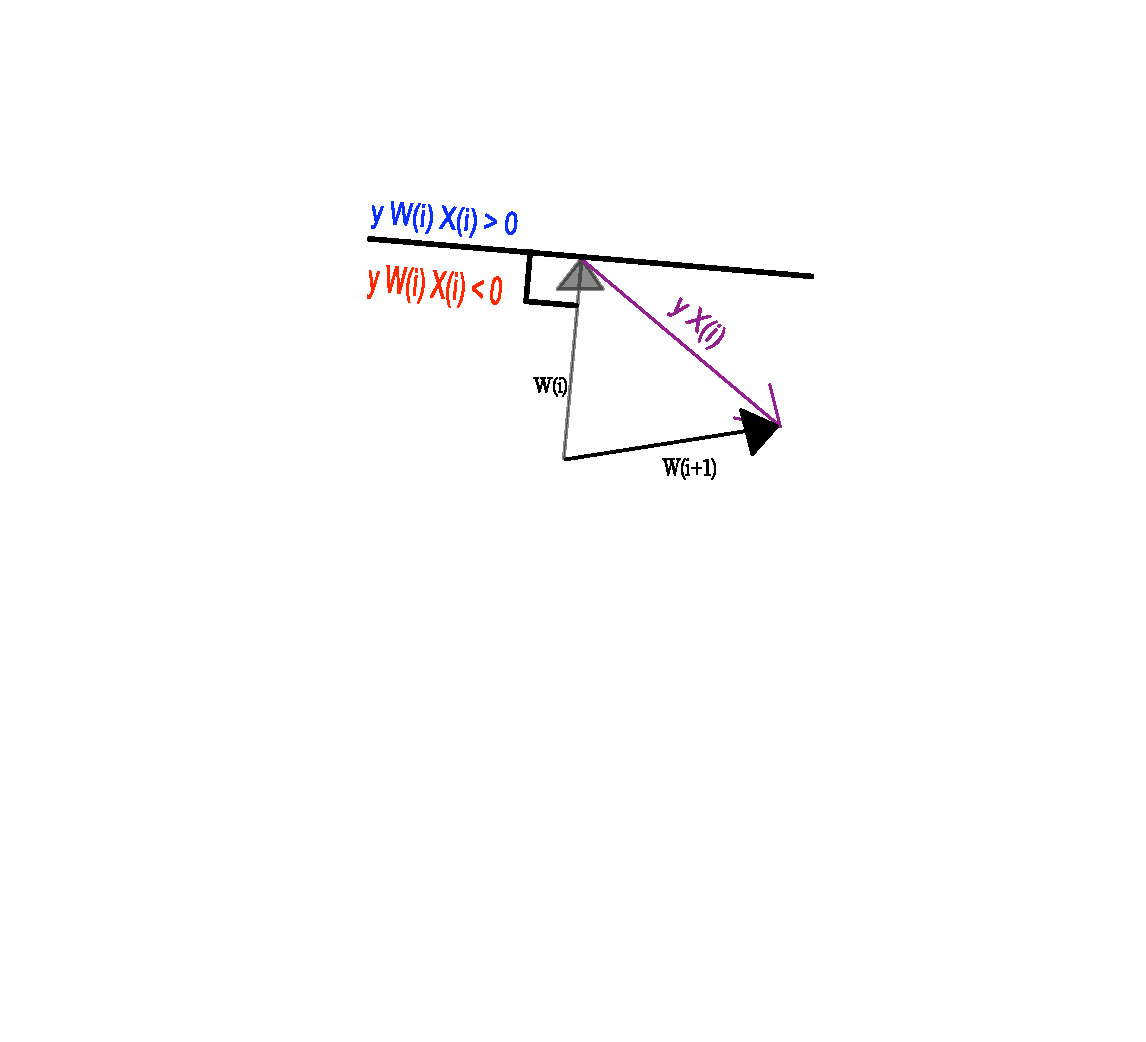
\includegraphics[height=10cm]{PerceptronAnim/PerceptronError.pdf}
\end{frame}

\begin{frame}
\frametitle{Upper bound on $\| \W_i \|$}
\pause
Proof by induction
\begin{itemize}
\item Claim: $ \| \W_{i} \|^2 \leq i R^2 $
\item Base: $i=0$, $\|\W_0\|^2 = 0$
\item Induction step (assume for $i$ and prove for $i+1$):\\
$ \| \W_{i+1} \|^2 \leq \|\W_i\|^2 + \|\X_i\|^2 $ \\
$\leq \|\W_i\|^2 + R^2 \leq (i+1) R^2$

\end{itemize}
\end{frame}

\begin{frame}
\frametitle{Lower bound on $\| \W_i \|$}
\pause
$\|\W_i\| \geq \W_{i} \cdot \V$ because $\| \V \|=1$.\\
\pause
We prove a lower bound on $\W_{i} \cdot \V$ using induction over $i$
\begin{itemize}
\item Claim: $ \W_{i} \cdot \V \geq i g $
\item Base: $i=0$, $\W_0 \cdot \V = 0$
\item Induction step (assume for $i$ and prove for $i+1$):\\
$ \W_{i+1} \cdot \V  = \left( \W_i + \X_i y_i \right) \V$
\pause
$= \W_i \cdot \V + y_i \X_i \cdot \V$ \\
$\geq i g + g = (i+1) g$
\end{itemize}
\end{frame}

\begin{frame}
\frametitle{Combining the upper and lower bounds}
~\\
~\\
\pause
$$(ig)^2 \leq \|\W_i\|^2 \leq i R^2$$
\pause
Thus:
$$ i \leq \left(\frac{R}{g} \right)^2 $$
\end{frame}

%\iffalse %%%%%%%%%%%%%%%%%%%%%%%%%%%%%%%%%%%%%%%%%%%%%%%%%%%%%%%%%%%%%%%%%%
\section{Laplace law of succession}

\begin{frame}
\frametitle{Estimating the bias of a coin}

\begin{itemize}
\item We observe $n$ coin flips:\\
{\bf H,T,T,H,H,T,H,T,T}
\item
We want to estimate the {\bf probability} that the next flip will be {\bf H}ead.
\item
Natural Answer:
\[
\frac{\#\mbox{\bf H}}{n} = \frac{4}{9}
\]
\end{itemize}
\end{frame}

\begin{frame}
\frametitle{What if the estimation has to be done online?}

\begin{itemize}
\item We observe a {bf sequence} of coin flips, and have to predict the probability of {\bf H}ead at each step:
\\ $p_0$,\pause 
{\bf H},\pause 
$p_1$,\pause
{\bf T},\pause
$p_2$,\pause 
$\ldots$
\item
What would be a good value for $p_0$?
\item
For $p_1$?
\item
Laplace Law of succession
\[
\frac{\#\mbox{\bf H} +1}{n+2}
\]
\item 
Turns out that a better rule is 
\[
\frac{\#\mbox{\bf H} +1/2}{n+1}
\]
Krichevsky and Trofimov, 1981
\item
Why? 
\item 
What does ``better'' mean?
\end{itemize}
\end{frame}

\begin{frame}
\frametitle{To be continued...}
Please
\begin{itemize}
\item Register on twiki (follow directions on my home page)
\item Follow link from main twiki page to ``Online learning course''
\item Add yourself to the list and the table on {\tt ClassParticipants}
\item Go to {\tt CoursePlan/LessonNo1} to see slides and to post questions and answers.
\item See you on Thursday!
\end{itemize}
\end{frame}
%\fi %%%%%%%%%%%%%%%%%%%%%%%%%%%%%%%%%%%%%%%%%%%%%%%%%%%%%%%%%%%%%%%%%%%

\end{document}


